\documentclass[12pt]{article}
\usepackage[margin=1in]{geometry}
\usepackage{amsmath,amsthm,amssymb,amsfonts}
\usepackage{graphicx}
\usepackage{physics}
%\usepackage{halloweenmath}
\usepackage{setspace}
\usepackage[font=small,labelfont=bf]{caption}

\newcommand{\N}{\mathbb{N}}
\newcommand{\Z}{\mathbb{Z}}

\newenvironment{part}[2][Part]{\begin{trivlist}
\item[\hskip \labelsep {\bfseries #1}\hskip \labelsep {\bfseries #2.}]}{\end{trivlist}}
%If you want to title your bold things something different just make another thing exactly like this but replace "problem" with the name of the thing you want, like theorem or lemma or whatever

\graphicspath{ {./} }

\begin{document}

\title{\textbf{ASTR 522: SED Fitting Lab}}
\author{Jonas Powell}
\maketitle


%\twocolumn
\begin{onehalfspacing}




\raggedright{\textbf{\Large Part 1:}}\\
\raggedright{\textbf{\large Plotting the SED of a Quasar}}

\begin{figure}[h!]
    \centering
    \begin{minipage}{0.48\textwidth}
        \centering
        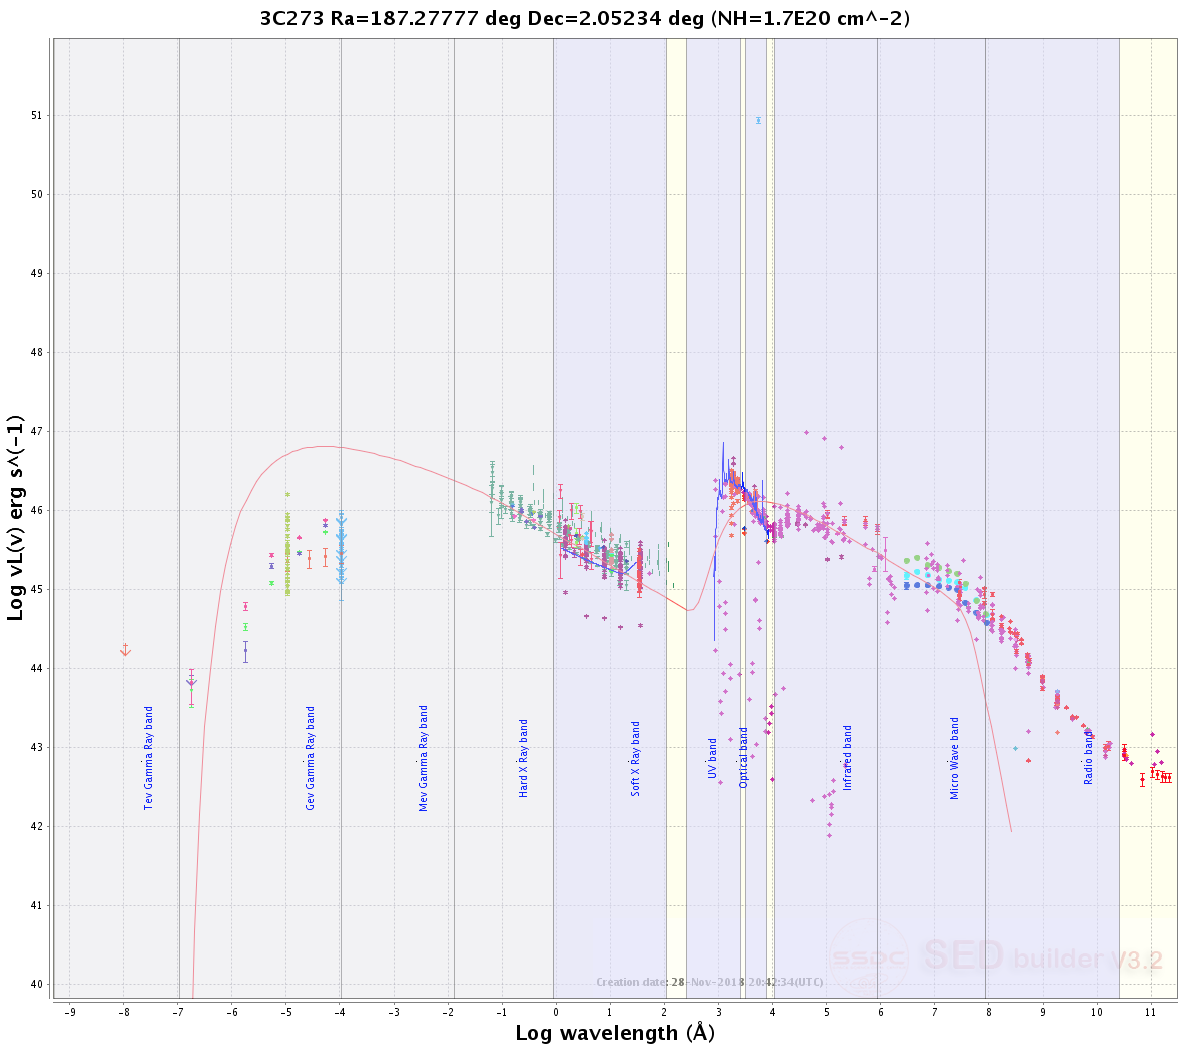
\includegraphics[width=1.05\textwidth]{part1} % first figure itself
        \caption{SED for the quasar 3C273.}
    \end{minipage}\hfill
    %\iffalse
    \begin{minipage}{0.48\textwidth}
        \centering
        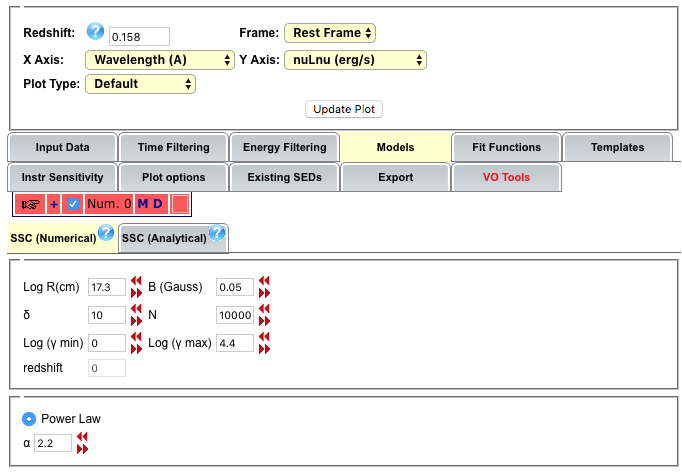
\includegraphics[width=0.75\textwidth]{part1_params} % second figure itself
        \caption{SED for the quasar 3C273 with Composite QSO template applied and ARO=0.61}
    \end{minipage}\hfill
  %\fi
\end{figure}

We see that there are two primary gaps in the data: one around the UV band and one between the end of the hard X-ray and the beginning of the GeV $\gamma$-ray band. Since we know that these data may be understood as showing two SEDs - one of the quasar itself (in the higher energy regime) and one of the quasar's disk - then we may recognize that the gap around the UV band exists because that is where the disk's SED falls off but the quasar's SED hasn't yet really started to contribute. The other gap represents a lack of telescopes that observe in that energy band.




\raggedright{\textbf{\Large Part 2:}}\\
\raggedright{\textbf{\large Plotting the SED of a Galaxy}}


z = H0 * d/c = 1.94e-3















\end{onehalfspacing}

\end{document}
